\documentclass[a4paper,12pt]{extarticle}
\usepackage[utf8x]{inputenc}
\usepackage[T1,T2A]{fontenc}
\usepackage[russian]{babel}
\usepackage{hyperref}
\usepackage{indentfirst}
\usepackage{listings}
\usepackage{color}
\usepackage{here}
\usepackage{array}
\usepackage{multirow}
\usepackage{graphicx}
\usepackage{amsmath}
\usepackage{amssymb}

\usepackage{caption}
\renewcommand{\lstlistingname}{Программа} % заголовок листингов кода

\bibliographystyle{ugost2008ls}

\usepackage{listings}
\lstset{ %
extendedchars=\true,
keepspaces=true,
language=C,						% choose the language of the code
basicstyle=\footnotesize,		% the size of the fonts that are used for the code
numbers=left,					% where to put the line-numbers
numberstyle=\footnotesize,		% the size of the fonts that are used for the line-numbers
stepnumber=1,					% the step between two line-numbers. If it is 1 each line will be numbered
numbersep=5pt,					% how far the line-numbers are from the code
backgroundcolor=\color{white},	% choose the background color. You must add \usepackage{color}
showspaces=false				% show spaces adding particular underscores
showstringspaces=false,			% underline spaces within strings
showtabs=false,					% show tabs within strings adding particular underscores
frame=single,           		% adds a frame around the code
tabsize=2,						% sets default tabsize to 2 spaces
captionpos=t,					% sets the caption-position to top
breaklines=true,				% sets automatic line breaking
breakatwhitespace=false,		% sets if automatic breaks should only happen at whitespace
escapeinside={\%*}{*)},			% if you want to add a comment within your code
postbreak=\raisebox{0ex}[0ex][0ex]{\ensuremath{\color{red}\hookrightarrow\space}},
texcl=true,
inputpath=listings,                     % директория с листингами
}

\usepackage[left=2cm,right=2cm,
top=2cm,bottom=2cm,bindingoffset=0cm]{geometry}

%% Нумерация картинок по секциям
\usepackage{chngcntr}
\counterwithin{figure}{subsection}
\counterwithin{table}{section}

%%Точки нумерации заголовков
\usepackage{titlesec}
\titlelabel{\thetitle.\quad}
\usepackage[dotinlabels]{titletoc}

%% Оформления подписи рисунка
\addto\captionsrussian{\renewcommand{\figurename}{Рис.}}
\captionsetup[figure]{labelsep = period}

%% Подпись таблицы
\DeclareCaptionFormat{hfillstart}{\hfill#1#2#3\par}
\captionsetup[table]{format=hfillstart,labelsep=newline,justification=centering,skip=-10pt,textfont=bf}

%% Путь к каталогу с рисунками
\graphicspath{{fig/}}

\setcounter{tocdepth}{3}

\begin{document}	% начало документа

% Титульная страница
\begin{titlepage}	% начало титульной страницы

	\begin{center}		% выравнивание по центру

		\large Санкт-Петербургский Политехнический Университет Петра Великого\\
		\large Институт компьютерных наук и технологий \\
		\large Кафедра компьютерных систем и программных технологий\\[6cm]
		% название института, затем отступ 6см
		
		\huge Телекоммуникационные технологии\\[0.5cm] % название работы, затем отступ 0,5см
		\large Отчет по лабораторной работе №6\\[0.1cm]
		\large Цифровая модуляция\\[5cm]

	\end{center}


	\begin{flushright} % выравнивание по правому краю
		\begin{minipage}{0.25\textwidth} % врезка в половину ширины текста
			\begin{flushleft} % выровнять её содержимое по левому краю

				\large\textbf{Работу выполнил:}\\
				\large Болдырев А.В.\\
				\large {Группа:} 33501/3\\
				
				\large \textbf{Преподаватель:}\\
				\large Богач Н.В.

			\end{flushleft}
		\end{minipage}
	\end{flushright}
	
	\vfill % заполнить всё доступное ниже пространство

	\begin{center}
	\large Санкт-Петербург\\
	\large \the\year % вывести дату
	\end{center} % закончить выравнивание по центру

\thispagestyle{empty} % не нумеровать страницу
\end{titlepage} % конец титульной страницы

\vfill % заполнить всё доступное ниже пространство

% Содержание
% Содержание
\renewcommand\contentsname{\centerline{Содержание}}
\tableofcontents
\newpage

 
\section{Цель работы}
Изучение методов модуляции цировых сигналов.
 
\section{Постановка задачи}
\begin{enumerate}
\item Получить сигналы BPSK, PSK, OQPSK, genQAM, MSK, M-FSK модуляторов.
\item Построить их сигнальные созвездия.
\item Провести сравнение изученных методов модуляции цифровых сигналов.
\end{enumerate}


\section{Теоретическая информация}

\subsection{Модуляция}
Сигналы от любых источников информации передаются по линиям связи к приемникам, например, в измерительно-вычислительные системы регистрации и обработки данных. Как правило, информационные сигналы являются низкочастотными и ограниченными по ширине спектра, тогда как методы передачи сигналов рассчитаны на работу с высокочастотным сигналом. При этом важным вопросом является частотное разделение каналов передачи информации с целью эффективного использования каналообразующего оборудования и выделенного для передачи частотного диапазона. Перенос спектра сигналов из низкочастотной области на заданную частоту, т.е. в выделенную для их передачи область высоких частот выполняется операцией \textit{модуляции}. Обозначим низкочастотный сигнал, подлежащий передаче по какому-либо каналу связи, $s(t)$ .   

В канале связи для передачи данного сигнала выделяется определенный диапазон высоких частот и формируется вспомогательный периодический высокочастотный сигнал $u(t)   =   f(t;   a_1,   a_2,   ...   a_m)$. Совокупность параметров $a_i$ определяет форму вспомогательного сигнала. Значения параметров $a_i$ в отсутствие модуляции являются величинами постоянными. Если на один из этих параметров перенести сигнал $s(t)$, т.е. сделать его значение пропорционально зависимым от значения $s(t)$ во времени (или по любой другой независимой переменной), то форма сигнала $u(t)$ приобретает новое свойство. Она служит для переноса информации, содержащейся в сигнале $s(t)$. Сигнал $u(t)$ называется \textit{несущим сигналом}, \textit{несущим колебанием} или просто \textit{несущей}  ($carrier$),  а физический процесс переноса информации на
параметры несущего сигнала     –     его \textit{модуляцией}. 

Исходный информационный сигнал $s(t)$ называют \textit{модулирующим}, результат модуляции    –    \textit{модулированным сигналом}. Обратную операцию выделения модулирующего сигнала из модулированного колебания называют демодуляцией или детектированием.

\subsection{Типы цифровой модуляции}
\subsubsection{BPSK, PSK}
BPSK и PSK - модуляция со сдвиглм фазы сигнала без изменения амплитуды. В PSK их может быть множество, в BPSK - один (на $\pi$).

Изображения сигнального созвездия и схемы модулятора BPSK приведены ниже на следующих рисунках:
\begin{figure}[H]
	\begin{center}
		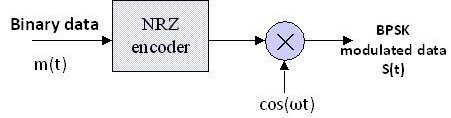
\includegraphics[width=1\linewidth]{BPSK_Scheme_theor.png}
		\caption{Схема устройства модулятора BPSK.} %% подпись к рисунку
		\label{BPSK_Scheme_theor} %% метка рисунка для ссылки на него
	\end{center}
\end{figure}
\begin{figure}[H]
	\begin{center}
		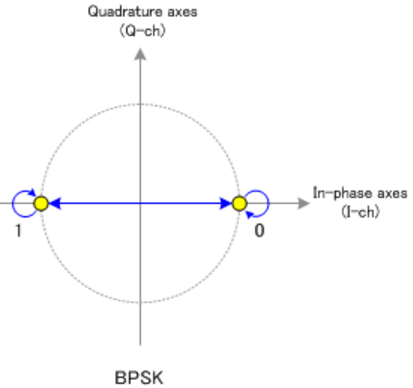
\includegraphics[width=0.5\linewidth]{BPSK_Sig_Con_theor.png}
		\caption{Сигнальное созвездие BPSK.} %% подпись к рисунку
		\label{BPSK_Sig_Con_theor} %% метка рисунка для ссылки на него
	\end{center}
\end{figure}

\subsubsection{genQAM, OQPSK}
При квадратурной амплитудной модуляции (КАМ) изменяется как фаза, так и амплитуда несущего сигнала. Это позволяет увеличить количество кодируемых в единицу времени бит и при этом повысить помехоустойчивость их передачи по каналу связи. В настоящее время число кодируемых информационных бит на одном интервале может достигать 8-9, а число состояний сигнала в сигнальном пространстве, соответственно – 256…512.
Квадратурное представление сигнала заключается в выражении колебания линейной комбинацией двух ортогональных составляющих – квадратурной и синфазной:
\begin{equation}
	S(t) = x(t) sin(\omega t + \varphi) cos(\omega t + \varphi)
\end{equation}
где x(t) и y(t) – биполярные дискретные сигналы.

Рассмотрим работу квадратурного модулятора на примере схемы формирования сигналов четырехфазной ФМ из битового потока. Исходная последовательность двоичных символов при помощи регистра сдвига разделяется на нечетные y и четные x импульсы, которые поступают на входы формирователей манипулирующих импульсов (ФМИ) квадратурного и синфазного каналов. На выходах ФМИ образуются последовательности биполярных импульсов $x(t)$ и $y(t)$ с амплитудой $\pm U_m$ и длительностью $2Т$, которые поступают на входы канальных перемножителей, где они независимо друг от друга модулируют по амплитуде два одинаковых несущих колебания, имеющих сдвиг фаз $90°$, т.е. находящихся в квадратуре. В результате, на их выходах формируются двухфазные $(0, \pi)$ колебания.
После суммирования они образуют сигнал ФМ-4 или квадратурный ФМ-сигнал (Quadrature Phase Shift Keying – QPSK). Поскольку в каждом канале осуществляется амплитудная манипуляция, этот вид модуляции называют еще квадратурной амплитудной манипуляцией (QASK – Quadrature Amplitude Shift Keying) или просто квадратурной амплитудной модуляцией (КАМ). При одновременной смене символов в обоих каналах модулятора (с 10 на 01, или с 00 на 11) в сигнале ФМ-4 происходит скачок фазы на $180° (\pi)$. Такие скачки фазы вызывают появление высокочастотных составляющих в спектре модулированного сигнала. В результате этого при прохождении сигнала через узкополосный фильтр возникают провалы огибающей несущего колебания до нуля. Такие изменения сигнала нежелательны, поскольку приводят к увеличению энергии боковых полос и помех в канале связи.
Четырехфазная ФМ со сдвигом (OQPSK – Offset QPSK) позволяет избежать скачков фазы на 180° и, следовательно, глубокой модуляции огибающей. Формирование сигнала в модуляторе OQPSK происходит так же, как и в модуляторе ФМ-4, за исключением того, что манипуляционные элементы информационных последовательностей $x(t)$ и $y(t)$ смещены во времени на длительность одного элемента $Т$, Pic. Изменение фазы при таком смещении модулирующих потоков определяется лишь одним элементом последовательности, а не двумя, как при ФМ 4. В результате скачки фазы на 180° отсутствуют, так как каждый элемент последовательности, поступающий на вход модулятора синфазного или квадратурного канала, может вызвать изменение фазы на $0$, $+90°$ или $-90°$.
\begin{figure}[H]
	\begin{center}
		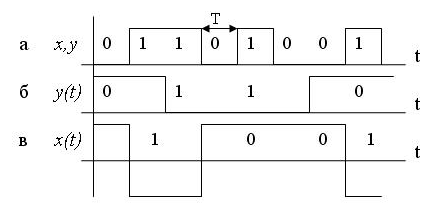
\includegraphics[width=1\linewidth]{manip_sig_theor.png}
		\caption{Формирование манипулирующих сигналов} %% подпись к рисунку
		\label{manip_sig_theor} %% метка рисунка для ссылки на него
	\end{center}
\end{figure} 

Преобразованные таким образом сигналы передаются в одном канале. Поскольку один и тот же физический канал используется для передачи двух сигналов, то скорость передачи КАМ-сигнала в отличие от АМ-сигнала в два раза выше.
Удобным способом визуализации сигналов модуляции можно считать их изображение векторами или точками в сигнальном пространстве. Совокупность сигнальных точек образует, так называемое, сигнальное созвездие (signal constellation).
Ниже показана структурная схема модулятора и диаграмма состояний (сигнальное созвездие) системы КАМ-16, в которой $x(t)$ и $y(t)$ принимают значения $\pm 1, \pm 3$ (4-х уровневая КАМ). 
\begin{figure}[H]
	\begin{center}
		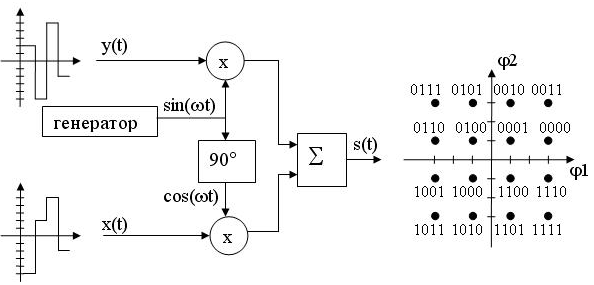
\includegraphics[width=1\linewidth]{QAM_16_theor.png}
		\caption{Модуляция КАМ-16 и ее сигнальное созвездие} %% подпись к рисунку
		\label{QAM_16_theor} %% метка рисунка для ссылки на него
	\end{center}
\end{figure} 

Существует несколько способов практической реализации 4-x уровневой КАМ. Еще одна схема, реализующая данный этот вид модуляции, использует два одинаковых 4 фазных модулятора. Структурная схема такого модулятора КАМ-16 имеет вид:
\begin{figure}[H]
	\begin{center}
		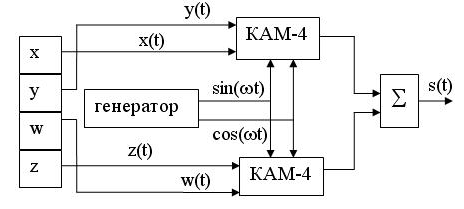
\includegraphics[width=1\linewidth]{QAM_Alt_Scheme_theor.png}
		\caption{Альтернативная схема модулятора КАМ-16} %% подпись к рисунку
		\label{QAM_Alt_Scheme_theor} %% метка рисунка для ссылки на него
	\end{center}
\end{figure} 

В общем случае, при формировании сигналов многопозиционной КАМ, модуляция ортогональных сигналов осуществляется в цифровом виде. Для этих целей используется два цифровых полосовых фильтра с одинаковой амплитудой входных колебаний, но различающихся фазовым сдвигом в 90о. Уровни усиления амплитуды для каждого потока устанавливают независимо. Для системы, поддерживающей m амплитудных уровней для каждого потока можно образовать m2 различных комбинаций нуля и единицы.
При равном числе точек в сигнальном созвездии спектр сигналов КАМ идентичен спектру сигналов ФМ. Однако помехоустойчивость систем ФМ и КАМ различна. При одинаковом числе точек сигналы системы КАМ имеют лучшую помехозащищенность, чем сигналы системы ФМ. Основная причина этого состоит в том, что расстояние между сигнальными точками в системе ФМ меньше расстояния между сигнальными точками в системе КАМ. Ниже представлены сигнальные созвездия систем КАМ-16 и ФМ-16 при одинаковой нормированной мощности сигнала.
\begin{figure}[H]
	\begin{center}
		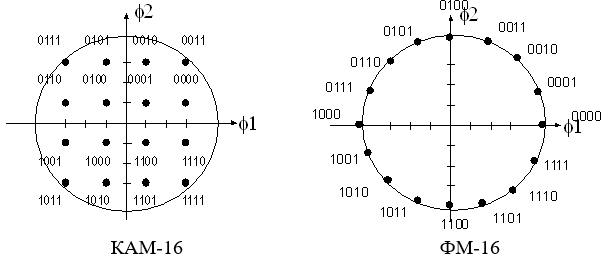
\includegraphics[width=1\linewidth]{QAM_sig_con_theor.png}
		\caption{Сигнальные созвездия КАМ-16 и ФМ-16} %% подпись к рисунку
		\label{QAM_sig_con_theor} %% метка рисунка для ссылки на него
	\end{center}
\end{figure} 

Расстояние между соседними точками сигнального созвездия в системе КАМ с L уровнями модуляции определяется выражением: 
\begin{equation}
	d = \frac {\sqrt{2}}{L - 1}
\end{equation}
Аналогично при ФМ:
\begin{equation}
	d = 2 sin(\frac{\pi}{M})
\end{equation}
где М – число фаз.

\subsubsection{MSK}
Частотная манипуляция с минимальным сдвигом (англ. Minimal Shift Keying (MSK)) представляет собой способ модуляции, при котором не происходит скачков фазы и изменение частоты происходит в моменты пересечения несущей нулевого уровня. MSK характеризуется тем, что значение частот соответствующих логическим «0» и «1» отличаются на величину равную половине скорости передачи данных. Другими словами, индекс модуляции равен 0,5.

Изображения сигнального созвездия и схемы модулятора MSK приведены ниже на риунках:
\begin{figure}[H]
	\begin{center}
		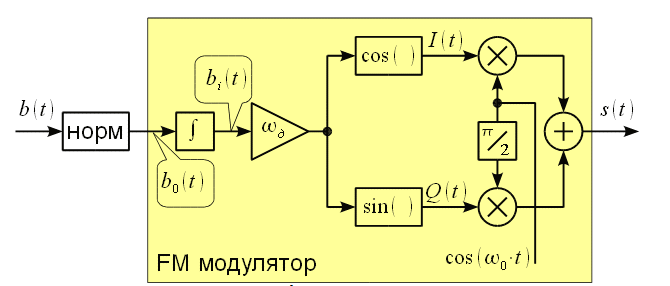
\includegraphics[width=1\linewidth]{MSK_scheme_theor.png}
		\caption{Структурная схема формирования MSK на основе FM модулятора.} %% подпись к рисунку
		\label{MSK_scheme_theor} %% метка рисунка для ссылки на него
	\end{center}
\end{figure}
\begin{figure}[H]
	\begin{center}
		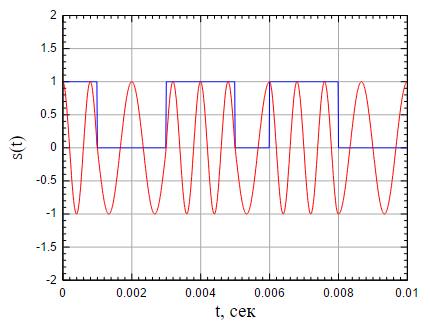
\includegraphics[width=1\linewidth]{MSK_sig_theor.png}
		\caption{Диаграмма MSK сигнала.} %% подпись к рисунку
		\label{MSK_sig_theor} %% метка рисунка для ссылки на него
	\end{center}
\end{figure}

\begin{figure}[H]
	\begin{center}
		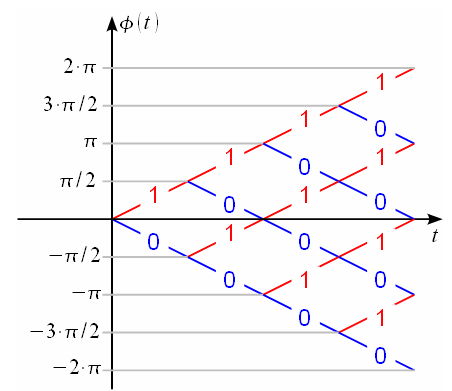
\includegraphics[width=1\linewidth]{MSK_diag_theor.png}
		\caption{Полная фазовая диаграмма при MSK для 4-х бит информации.} %% подпись к рисунку
		\label{MSK_diag_theor} %% метка рисунка для ссылки на него
	\end{center}
\end{figure}
\begin{figure}[H]
	\begin{center}
		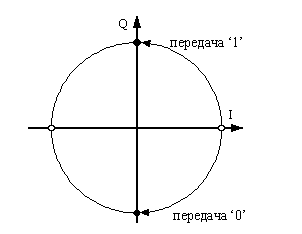
\includegraphics[width=0.5\linewidth]{MSK_sig_con_theor.png}
		\caption{Сигнальное созвездие MSK.} %% подпись к рисунку
		\label{MSK_sig_con_theor} %% метка рисунка для ссылки на него
	\end{center}
\end{figure}

\subsubsection{MFSK}
Можно построить и модулятор многопозиционной частотной модуляции. В этом случае будет использовано большее количество синусоидальных генераторов, а для управления коммутатором потребуется многоразрядное двоичное число.

Сигналы в многопозиционной частотной модуляции могут быть описаны в соответствии со следующим выражением:
\begin{equation}
	s_1 (t) =  cos(\omega_1 t); s_2 (t) =  cos(\omega_2 t); ...; s_N (t) =  cos(\omega_N t); 
\end{equation}
формула сигнала 1 многопозиционной частотной модуляции,  формула сигнала 2 многопозиционной частотной модуляции, …,  формула сигнала N многопозиционной частотной модуляции (3)
где $s_1$ используется для передачи первого состояния символа;
$s_2$ — для передачи второго состояния символа;
$s_N$ — для передачи N-го состояния символа.

Использование многопозиционной частотной модуляции позволяет реализовать высокочастотный сигнал с постоянной амплитудой. Такой сигнал позволяет строить радиопередатчики с максимальным кпд, так как при применении сигнала с постоянной амплитудой, усилитель мощности радиопередатчика работает в оптимальном режиме.

 На практике получила распространение двойная частотная модуляция — ДЧМ (C4FM) использующаяся в режиме с непрерывным изменением фазы сигнала. В этом виде модуляции используется четыре значения частоты несущего колебания. Таким количеством частот можно передать два символа в течение длительности одного символа.

Дальнейшее увеличение количества частот в радиоканале не имеет смысла, так как это приводит к неоправданному расширению спектра сигнала. Ширина спектра сигнала расширяется пропорционально количеству частот, а количество одновременно передаваемых бит растет пропорционально двоичному логарифму от количества использованных частот.


\section{Ход работы}
Цифровая модуляция и демодуляция включают в себя две стадии. При модуляции цифровое сообщение сначала преобразуется в аналоговый модулирующий сигнал с помощью функции modmap, а затем осуществляется аналоговая модуляция. При демодуляции сначала получается аналоговый демодулированный сигнал, а затем он преобразуется в цифровое сообщение с помощью функции demodmap.
 
Аналоговый несущий сигнал модулируется цифровым битовым потоком.
Существуют три фундаментальных типа цифровой модуляции (или шифтинга) и один гибридный:
\begin{enumerate}
\item ASK – Amplitude shift keying (Амплитудная двоичная модуляция).
\item FSK – Frequency shift keying (Частотая двоичная модуляция).
\item PSK – Phase shift keying (Фазовая двоичная модуляция).
\item ASK/PSK.
\end{enumerate}
Одна из частных реализаций схемы ASK/PSK - QAM - Quadrature Amplitude Modulation (квадратурная амплитудная модуляция (КАМ). Это метод объединения двух AM-сигналов в одном канале. Он позваляет удвоить эффективную пропускную способность. В QAM используется две несущих с одинаковой частотой но с разницей в фазе на четверть периода.
Частотная модуляция представляет логическую единицу интервалом с большей частотой, чем ноль.
Фазовый сдвиг представляет «0» как сигнал без сдвига, а «1» как сигнал со сдвигом.
BPSK использует единственный сдвиг фазы между «0» и «1» — 180 градусов, половина периода.
QPSK использует 4 различных сдвига фазы (по четверти периода) и может кодировать 2 бита в символе (01, 11, 00, 10).
 
Реализация различных типов модуляций с помощью MATLAB:

\lstinputlisting[
	label=code:DiscrMod2,
	caption={Код в МатЛаб},% для печати символ '_' требует выходной символ '\'
]{DiscrMod2.m}

Результаты выполнения представлены на рисунках ниже:

\subsection{BPSK-модуляция}
 
\begin{figure}[H]
	\begin{center}
		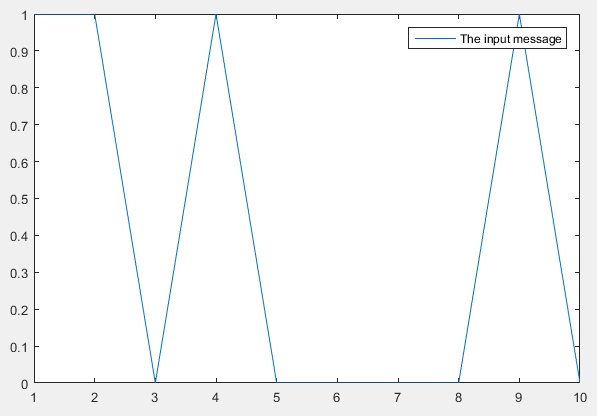
\includegraphics[width=0.5\linewidth]{Inp_msg_BPSK.png}
		\caption{Входной сигнал BPSK.} %% подпись к рисунку
		\label{Inp_msg_BPSK} %% метка рисунка для ссылки на него
	\end{center}
\end{figure}

\begin{figure}[H]
	\begin{center}
		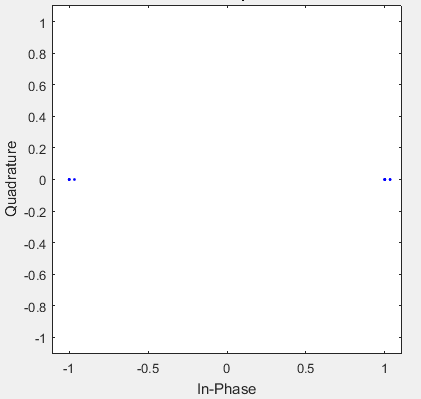
\includegraphics[width=0.5\linewidth]{sig_con_bpsk.png}
		\caption{Сигнальное созвездие BPSK.} %% подпись к рисунку
		\label{sig_con_bpsk} %% метка рисунка для ссылки на него
	\end{center}
\end{figure}

\begin{figure}[H]
	\begin{center}
		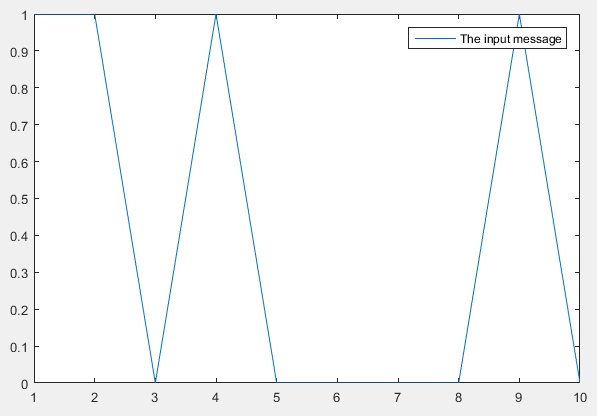
\includegraphics[width=0.5\linewidth]{Inp_msg_BPSK.png}
		\caption{Демодулированный сигнал BPSK.} %% подпись к рисунку
		\label{Inp_msg_BPSK} %% метка рисунка для ссылки на него
	\end{center}
\end{figure}

\subsection{PSK-модуляция}

\begin{figure}[H]
	\begin{center}
		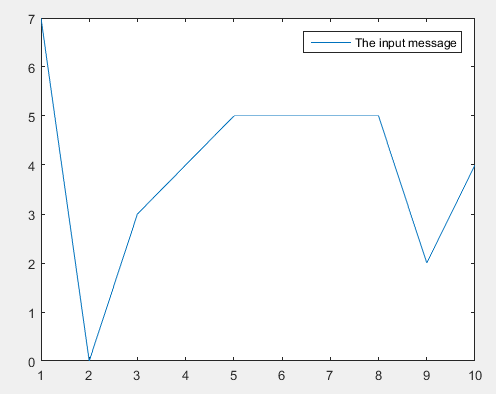
\includegraphics[width=0.5\linewidth]{Inp_msg_PSK.png}
		\caption{Входной сигнал PSK.} %% подпись к рисунку
		\label{Inp_msg_PSK} %% метка рисунка для ссылки на него
	\end{center}
\end{figure}
 
\begin{figure}[H]
	\begin{center}
		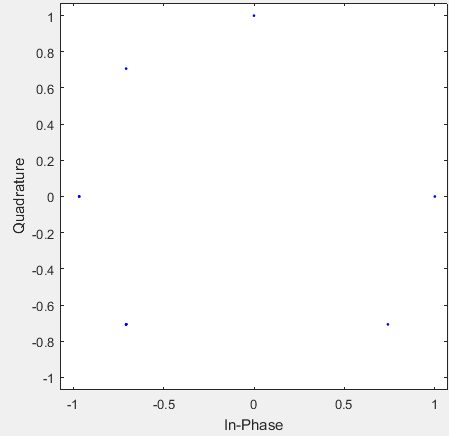
\includegraphics[width=0.5\linewidth]{sig_con_psk.png}
		\caption{Сигнальное созвездие PSK.}
		\label{sig_con_psk}
	\end{center}
\end{figure}

\begin{figure}[H]
	\begin{center}
		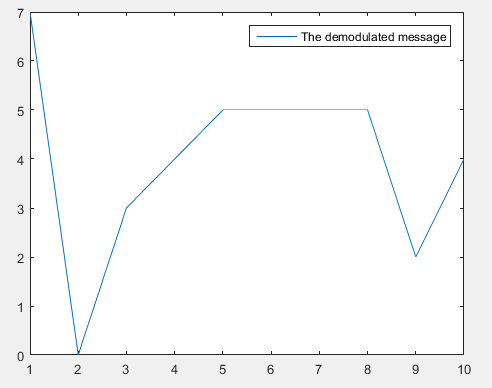
\includegraphics[width=0.5\linewidth]{Demod_msg_PSK.png}
		\caption{Демодулированный сигнал PSK.} %% подпись к рисунку
		\label{Demod_msg_PSK} %% метка рисунка для ссылки на него
	\end{center}
\end{figure}

\subsection{OQPSK-модуляция}

\begin{figure}[H]
	\begin{center}
		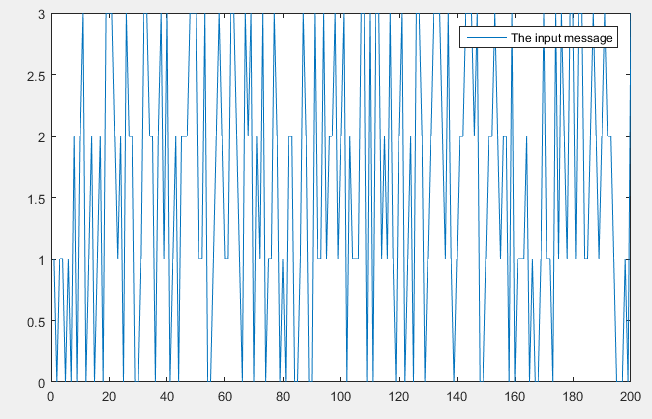
\includegraphics[width=0.5\linewidth]{Inp_msg_OQPSK.png}
		\caption{Входной сигнал OQPSK.} %% подпись к рисунку
		\label{Inp_msg_OQPSK} %% метка рисунка для ссылки на него
	\end{center}
\end{figure}

\begin{figure}[H]
	\begin{center}
		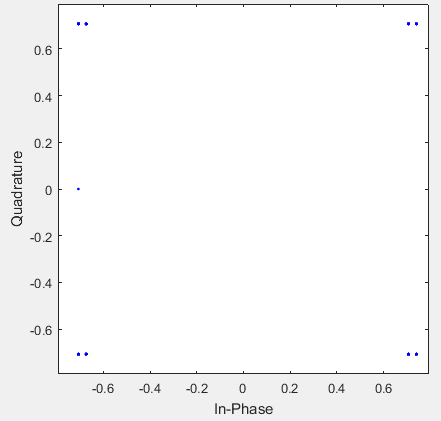
\includegraphics[width=0.5\linewidth]{sig_con_oqpsk.png}
		\caption{Сигнальное созвездие OQPSK.} %% подпись к рисунку
		\label{sig_con_oqpsk} %% метка рисунка для ссылки на него
	\end{center}
\end{figure}

\begin{figure}[H]
	\begin{center}
		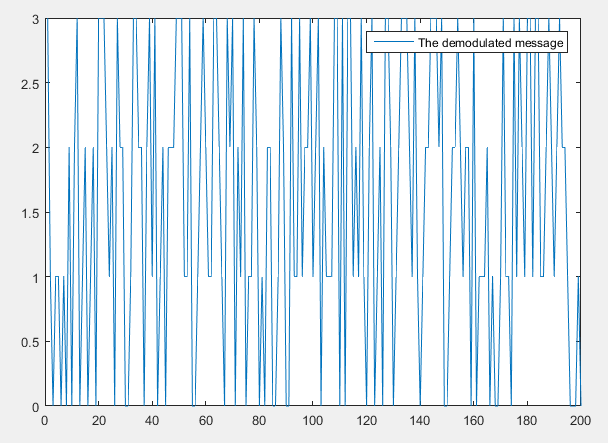
\includegraphics[width=0.5\linewidth]{Demod_msg_OQPSK.png}
		\caption{Демодулированный сигнал OQPSK.} %% подпись к рисунку
		\label{Demod_msg_OQPSK} %% метка рисунка для ссылки на него
	\end{center}
\end{figure}

\subsection{genQAM-модуляция}

\begin{figure}[H]
	\begin{center}
		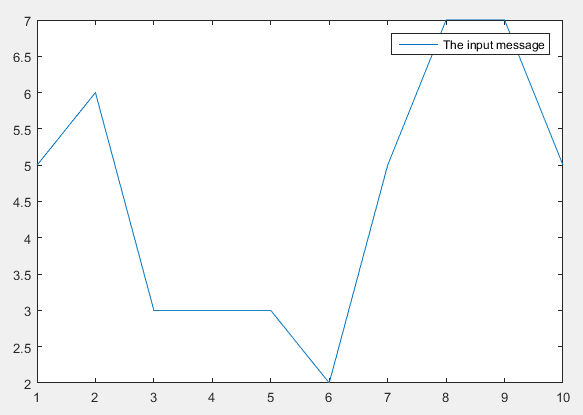
\includegraphics[width=0.5\linewidth]{Inp_msg_genQAM.png}
		\caption{Входной сигнал genQAM.} %% подпись к рисунку
		\label{Inp_msg_genQAM} %% метка рисунка для ссылки на него
	\end{center}
\end{figure}

\begin{figure}[H]
	\begin{center}
		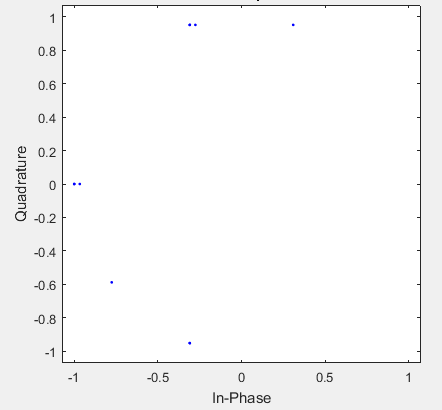
\includegraphics[width=0.5\linewidth]{sig_con_genqam.png}
		\caption{Сигнальное созвездие genQAM.}
		\label{sig_con_genqam}
	\end{center}
\end{figure}

\begin{figure}[H]
	\begin{center}
		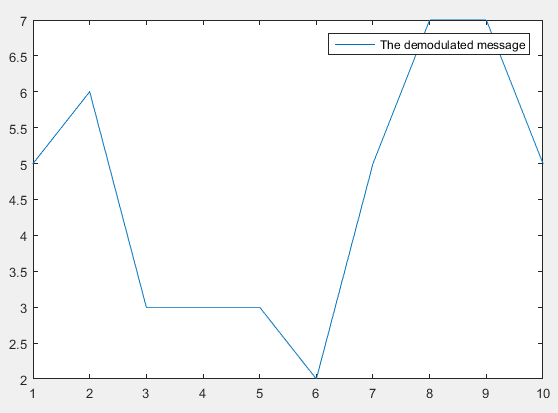
\includegraphics[width=0.5\linewidth]{Demod_msg_genQAM.png}
		\caption{Демодулированный сигнал genQAM.} %% подпись к рисунку
		\label{Demod_msg_genQAM} %% метка рисунка для ссылки на него
	\end{center}
\end{figure}

\subsection{MSK-модуляция}

\begin{figure}[H]
	\begin{center}
		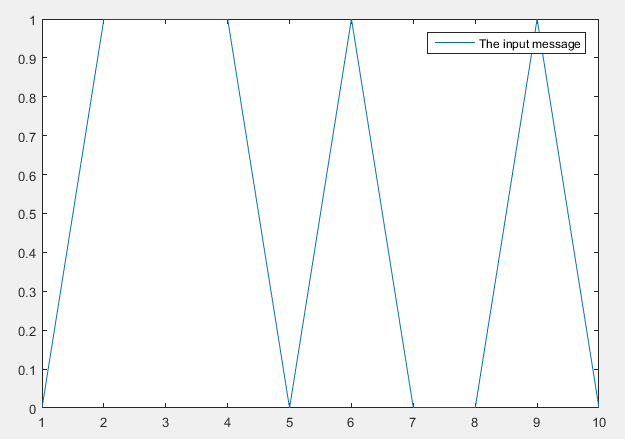
\includegraphics[width=0.5\linewidth]{Inp_msg_MSK.png}
		\caption{Входной сигнал MSK.} %% подпись к рисунку
		\label{Inp_msg_MSK} %% метка рисунка для ссылки на него
	\end{center}
\end{figure}

\begin{figure}[H]
	\begin{center}
		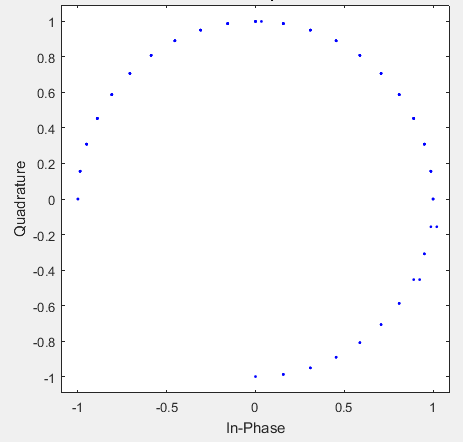
\includegraphics[width=0.5\linewidth]{sig_con_msk.png}
		\caption{Сигнальное созвездие MSK.} %% подпись к рисунку
		\label{sig_con_msk} %% метка рисунка для ссылки на него
	\end{center}
\end{figure}

\begin{figure}[H]
	\begin{center}
		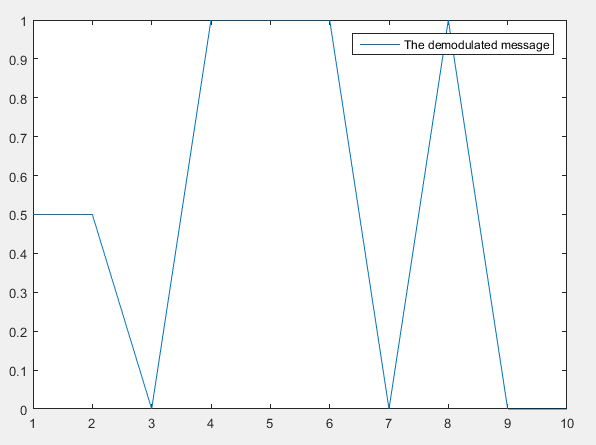
\includegraphics[width=0.5\linewidth]{Demod_msg_MSK.png}
		\caption{Демодулированный сигнал MSK.} %% подпись к рисунку
		\label{Demod_msg_MSK} %% метка рисунка для ссылки на него
	\end{center}
\end{figure}
Как можно видеть, при использовании MSK выходной сигнал имеет задержку при демодуляции.

\subsection{MFSK-модуляция}
В Simulink была построена модель MFSK-модулятора, результаты работы совпали с ожидаемыми, входная последовательность совпала с выходной.
\begin{figure}[H]
	\begin{center}
		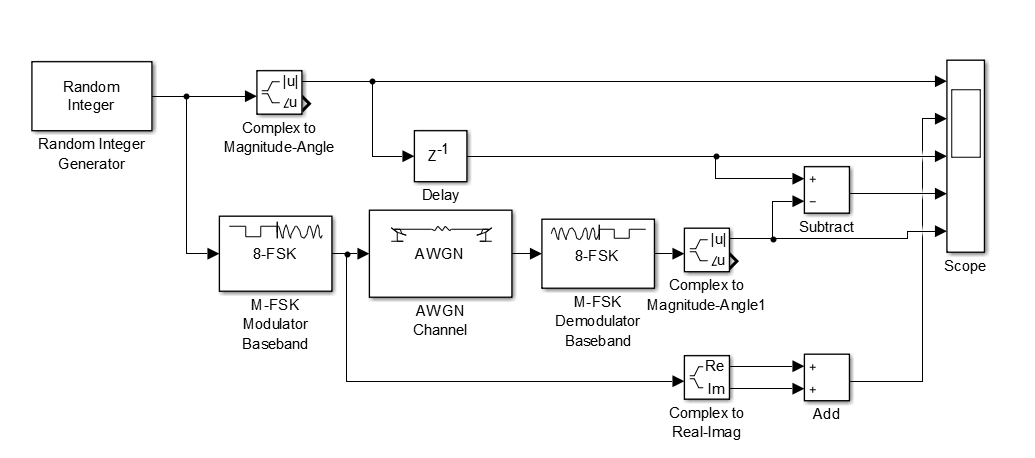
\includegraphics[width=1\linewidth]{MFSK_Mod_theor.png}
		\caption{Simulink-модель MFSK.} %% подпись к рисунку
		\label{MFSK_Mod_theor} %% метка рисунка для ссылки на него
	\end{center}
\end{figure}

\begin{figure}[H]
	\begin{center}
		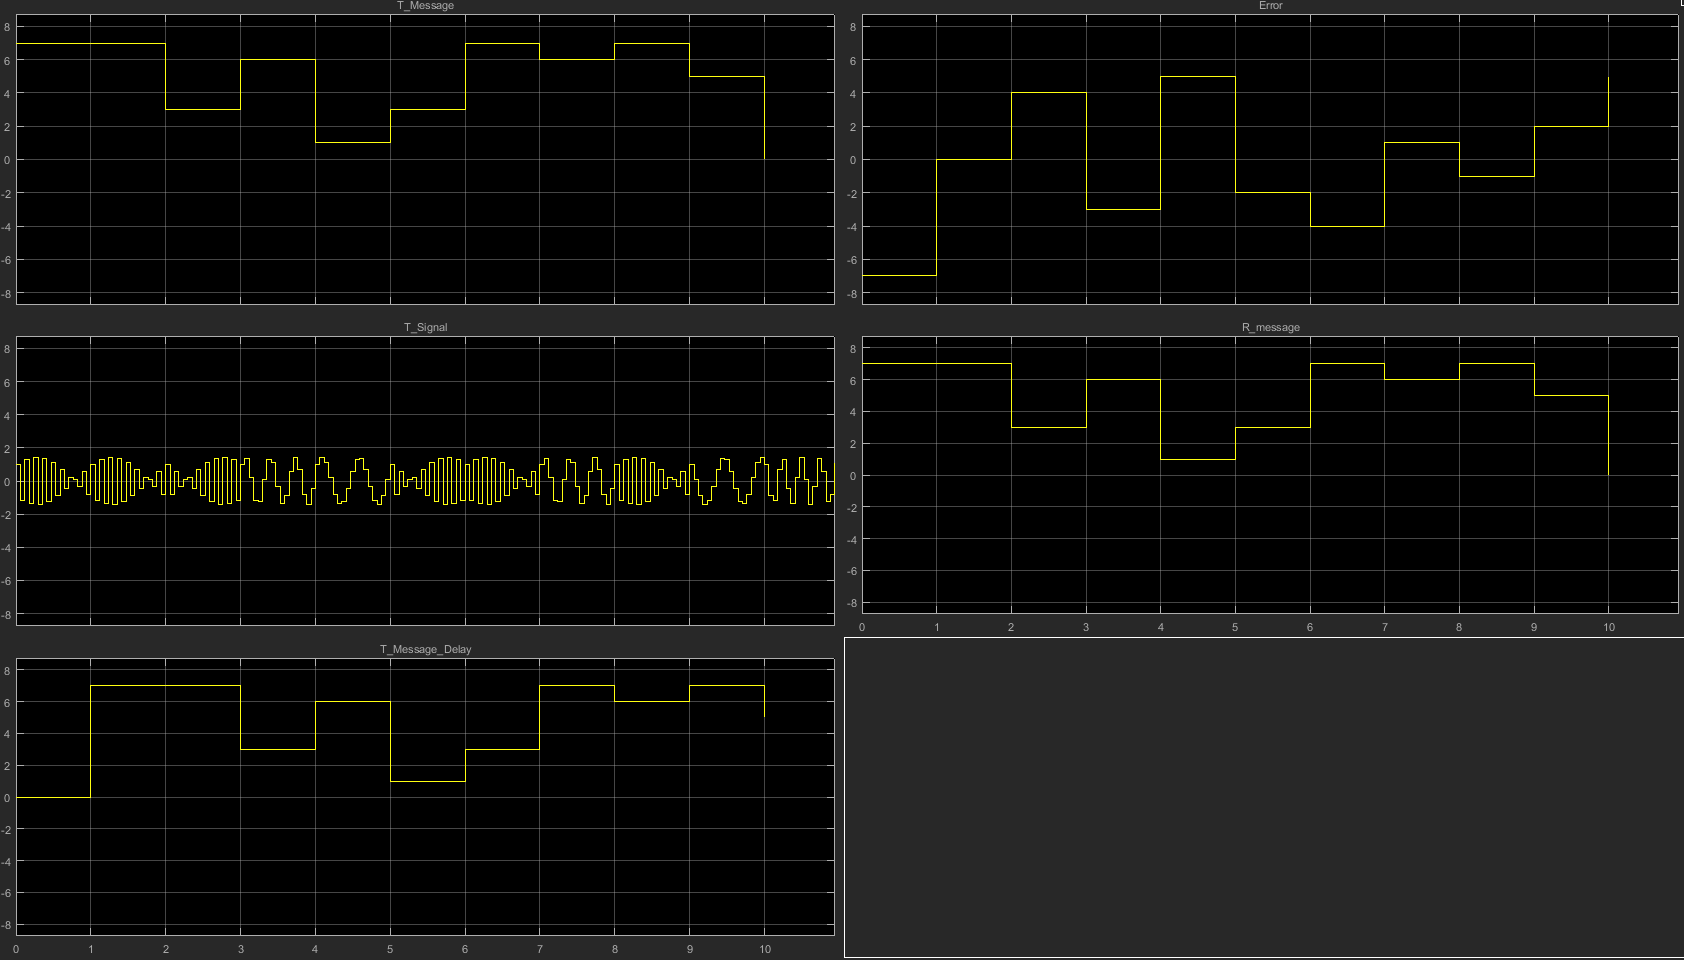
\includegraphics[width=1.1\linewidth]{MFSK_Gen.png}
		\caption{Графики входного сигнала, задержанного сигнала, модулированного сигнала, сигнала ошибки с задержанным сигналом, выходного сигнала MFSK.} %% подпись к рисунку
		\label{MFSK_Gen} %% метка рисунка для ссылки на него
	\end{center}
\end{figure}
  
 
\section{Выводы}
Цифровая модуляция — процесс преобразования последовательности кодовых символов в последовательность элементов целостного сигнала. Существуют следующие типы цифровой модуляции (манипуляции): частотная манипуляция, фазовая манипуляция, амплитудная манипуляция, квадратурная амплитудная манипуляция. 

Квадратурная амплитудная манипуляция (QAM) — манипуляция, при которой изменяется как фаза, так и амплитуда сигнала, что позволяет увеличить количество информации, передаваемой одним состоянием сигнала. 

Фазовая манипуляция (PSK) — один из видов фазовой модуляции, при которой фаза несущего колебания меняется скачкообразно в зависимости от информационного сообщения. 

Двоичная фазовая манипуляция — самая простая форма фазовой манипуляции. Работа схемы двоичной ФМн заключается в смещении фазы несущего колебания на одно из двух значений, нуль или $\pi$. Двоичную фазовую манипуляцию можно также рассматривать как частный случай квадратурной манипуляции (QAM-2). 

При квадратурной фазовой манипуляции (QPSK) используется созвездие из четырёх точек, размещённых на равных расстояниях на окружности. Имеется 4 фазовых смещений, при этом в QPSK на символ приходится два бита. 

Частотная манипуляция с минимальным сдвигом (MSK) представляет собой способ модуляции, при котором не происходит скачков фазы и изменение частоты происходит в моменты пересечения несущей нулевого уровня. Принцип MSK таков, что значение частот соответствующих логическим «0» и «1» отличаются на величину равную половине скорости передачи данных. Другими словами, индекс модуляции равен $0,5$. 

Уровень модуляции определяет количество состояний несущей, используемых для передачи информации. Чем выше этот уровень, тем большими скоростными возможностями и меньшей помехоустойчивостью обладает модуляция. Число бит, передаваемых одним состоянием, определяется как $Log (N)$, где N — уровень модуляции. Таким образом, чем выше уровень модуляции, тем больше данных мы можем передать (или потерять) за единицу времени.
\end{document}